\chapter{The choice of the sliding window} % Main chapter title

To study of the evolution of Stack Exchange communities, we chose to at each time step $t$ analyze the structure of interaction networks created in the period $[t, t+\tau)$. By this, we have better insight into how network properties evolve. However, it is not defined what value the sliding window should take. The previous studies showed that the value of a sliding window determines how much information is saved. If $\tau$ is small, sub-networks are sparse, while for a large sliding window, important changes in the measures may not be detected \cite{krings2012effects, arnold2021moving}. We analyze how network properties and dynamic reputation depend on the window size. For example, we use Astronomy and compare the active and closed communities. Similar conclusions can be observed for other pairs of communities. The time window of 30 days approximates the one month.  

We show the network properties for sub-networks of 10, 30, and 60 days sliding windows. For a sliding window of 10 days, results may be too noisy, and we may not observe some important trends in the community. The number of users for beta astronomy seems to fluctuate around some mean value. On the larger scale, 30 days window,  it is more apparent that the number of users slightly increases over time. Contrary, for too large an aggregation window (60 days), important information about the time series can be lost, such as the local minimum of the number of users around time step 80 that is observed for the 30-day sliding window. 
From network measures such as L/N and clustering, we conclude that the difference between closed and active sites is more transparent with a larger aggregation window. Still, on each scale, beta sites show a higher number of nodes, number of links per node and clustering coefficient.

As before, we study the structure of created sub-networks through the lens of core-periphery structure. On small scales, within the window of 10 days, there are often few or even no nodes in the core, and it can affect the calculation of other measures of interest. Such behaviour is more typical for closed communities. With the size of the sliding window, the number of nodes in the core increases and the results of core-periphery measures and dynamical reputation between core users and between core and periphery users becomes smoother. Finally, the choice of the sliding window does not change the conclusion that core users in the beta communities produce more activity and make a strong core. However, our main results are shown for a sliding window of 30 days, as it creates a good compromise between large and small time scales.   

\begin{figure}[h!]
	\centering
	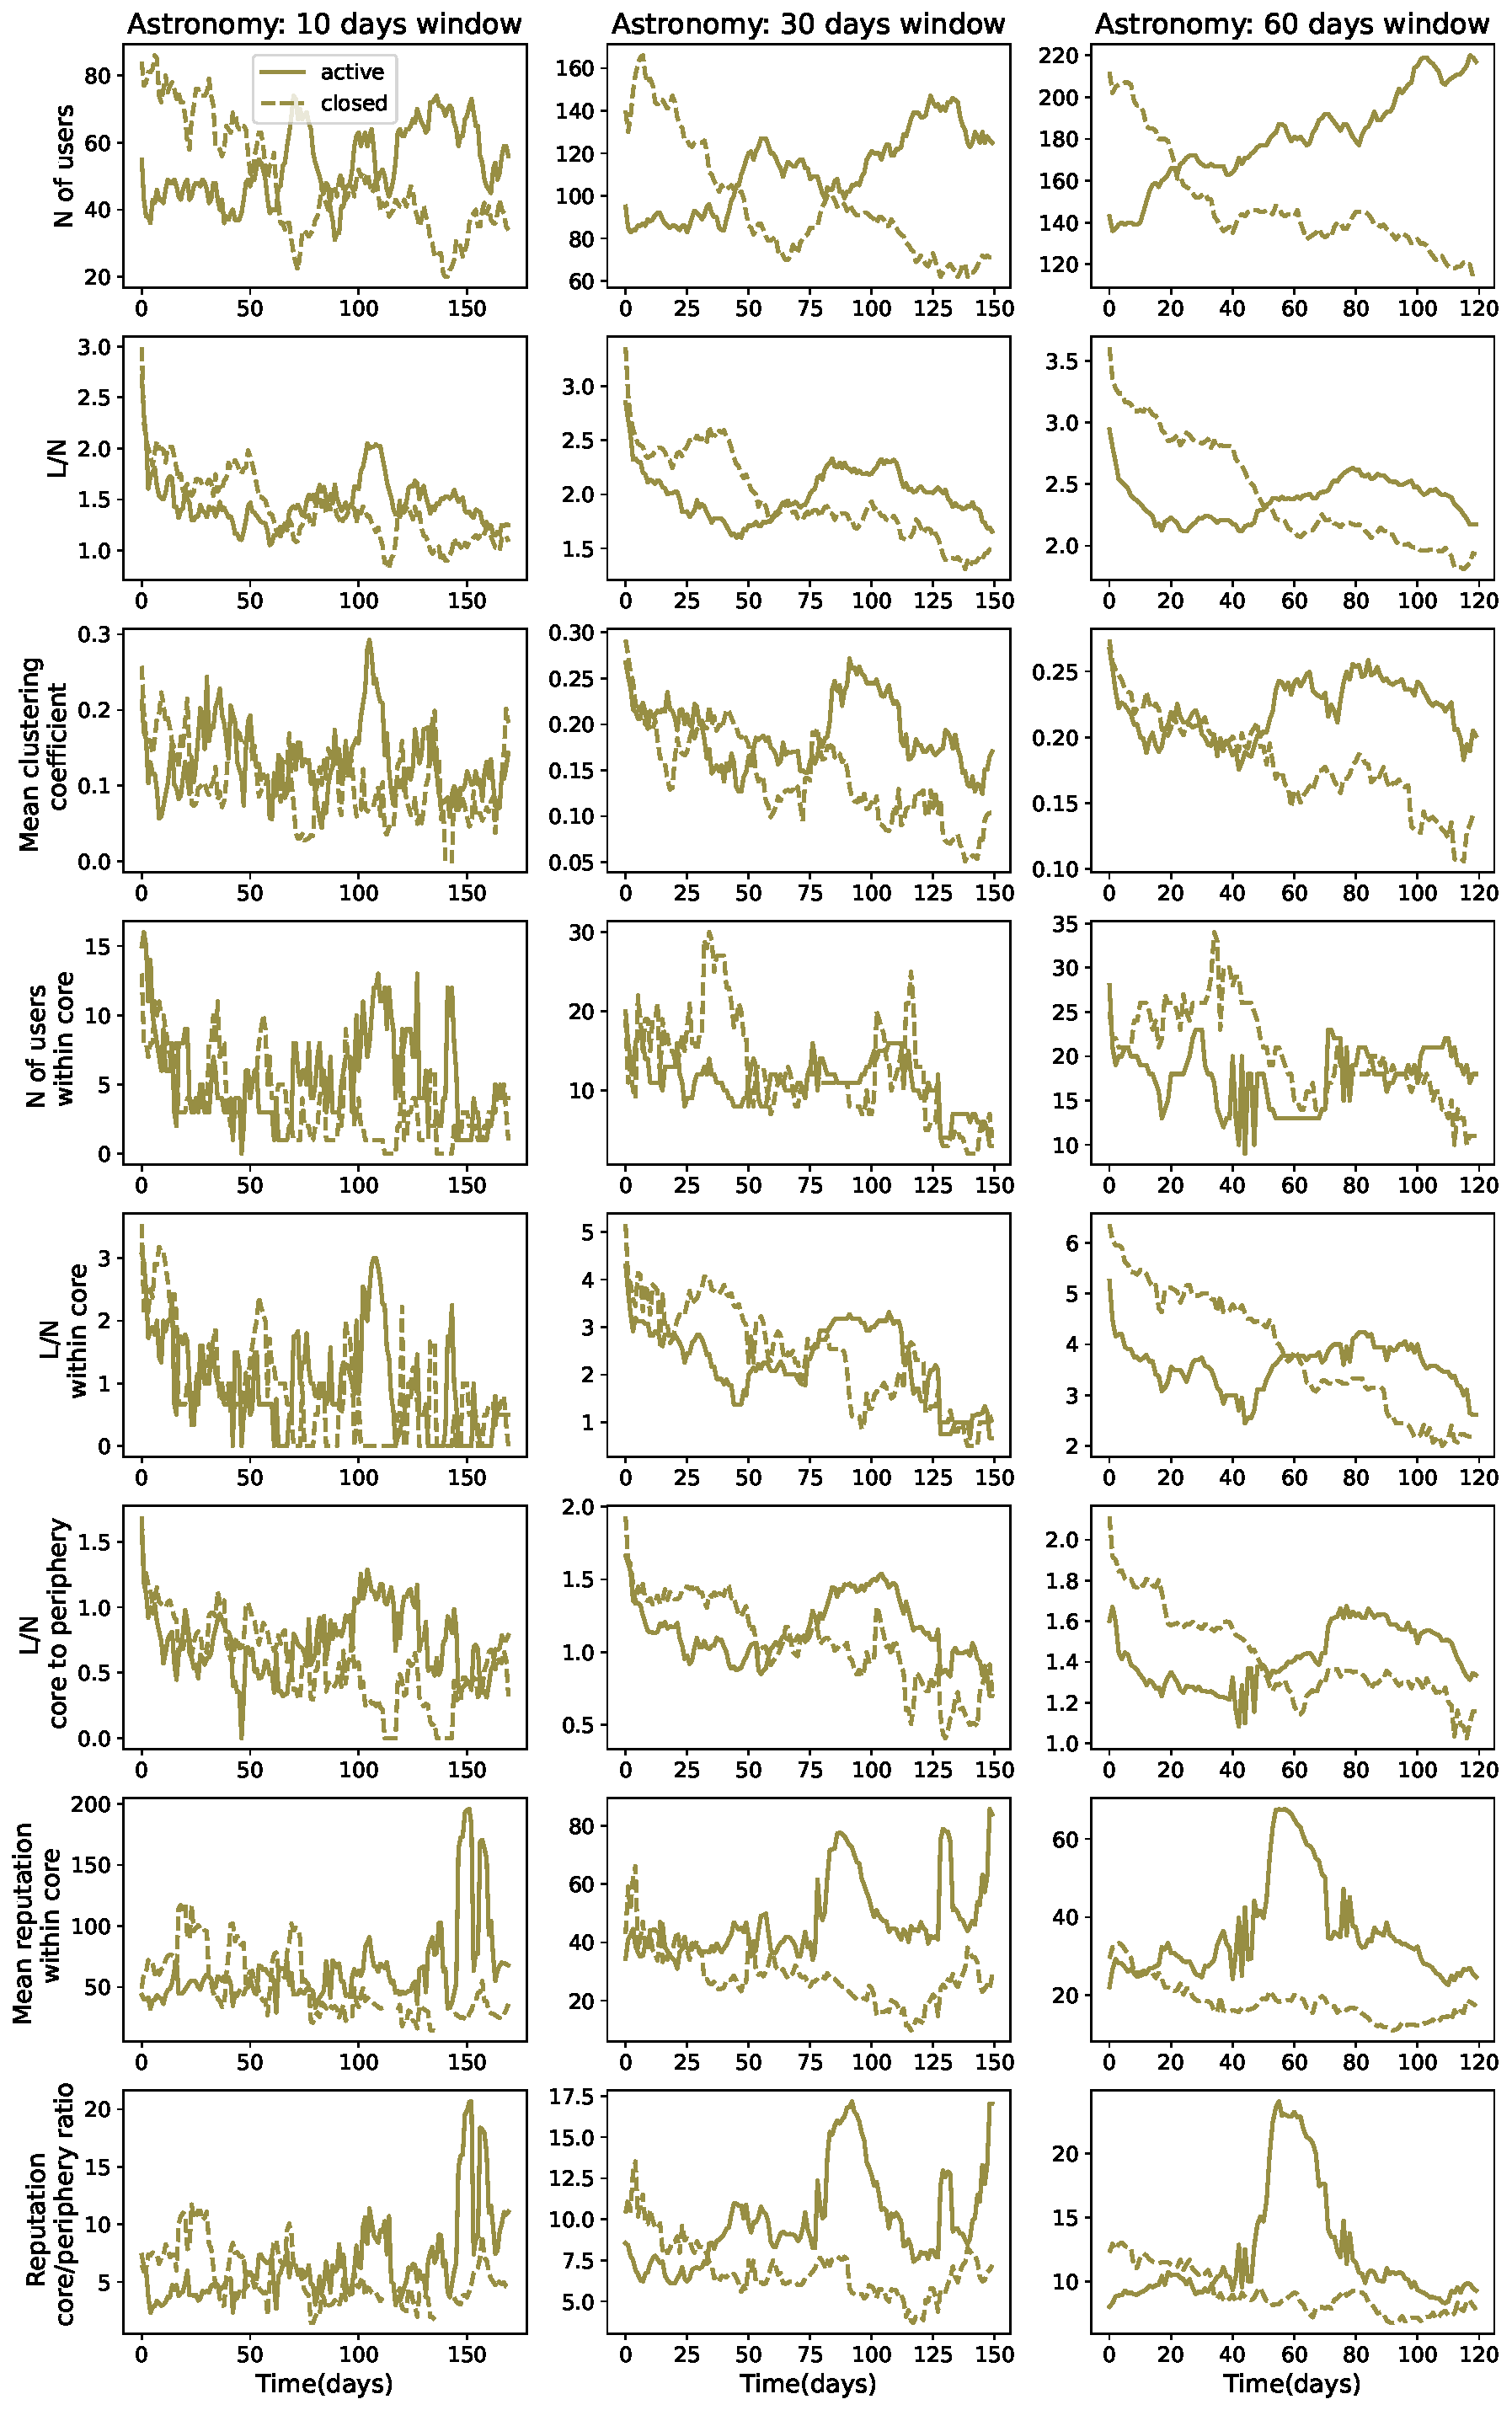
\includegraphics[width=0.9\linewidth]{figures/stackexchange/sliding_window.pdf}
	\caption{Results for different sliding windows. Example is for astronomy, blue solid lines- active, orange dashed lines - closed site. }
	\label{fig:windows}
\end{figure}
